\subsection{A Deep Architecture for Semantic Parsing \cite{Grefenstette2014}}

This paper presents a novel deep learning architecture which provides a semantic parsing system through the union of two neural models of language semantics. It allows for the generation of ontology-specific queries from natural language statements and questions without the need for parsing, which makes it especially suitable to grammatically malformed or syntactically atypical text such as tweets.

The goal of \emph{semantic parsing} is to map natural language sentences to formal representations of their underlying meaning. Within the context of question answering - the focus of this paper - semantic parsing typically aims to map natural language to database queries that would answer a given question.

The model proposed in the paper borrows from two approaches in the deep learning literature: the \emph{Bilingual Compositional Sentence Model (BiCVM)} and \emph{Conditional Neural Language Model (CNLM)}.

\begin{figure}[h]
  \centering
  % Requires \usepackage{graphicx}
  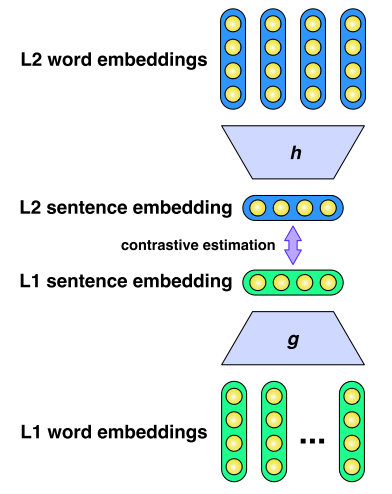
\includegraphics[width=.5\linewidth]{G2014-BiCVM.png}\\
  \caption{Diagrammatic representation of a BiCVM.}\label{fig:BiCVM}
\end{figure}

The BiCVM model shown in Figure \ref{fig:BiCVM} assumes vector composition functions $g$ and $h$, which map an ordered set of word embeddings onto a single vector. For semantically equivalent sentences $a, b$ across different languages (for example English and Chinese), the model aims to minimise the distance between these composed representations:
$$E_{bi}(a,b) = ||g(a) - h(b)||^2.$$
This error is combined with a noise-contrastive hinge loss, where $n$ is a randomly sampled sentence dissimilar to the parallel pair $\{a,b\}$, and $m$ denotes some margin:
$$E_{hl}(a,b,n) = max(0, m + E_{bi}(a,b) - E_{bi}(a,bn)).$$

A \emph{log-bilinear language model} is a neural network modelling a probability distribution over the next word in a sequence given the previous $n-1$, i.e. $p(w_n | w_{1:n-1})$. Let $C_i$ be the context transform matrix which modifies the representation of the $i$th word in the word history. Let $b_{w_i}$ be a scalar bias associated with a word $w_i$, and $b_R$ be a bias vector associated with the model. A log-bilinear model expressed the probability of $w_n$ as a function of the energy of the network:
$$E(w_n ; w_{1:n-1}) = -(\sum^{n-1}_{i=1}R_{w_i}^T C_i) R_{w_n} - b_R^T R_{w_n} - b_{w_n}.$$
To reframe a log-bilinear language model as a CNLM, the simplest way is to do this additively, which allows us to treat the contribution of the conditional variable $\beta$ as an extra word in the history.

The models described above can be combined to form a model capable of jointly learning a shared latent representation for question/query pairs using a BiCVM, and using this latent representation to learn a conditional log-bilinear CNLM.

\begin{figure}[h]
  \centering
  % Requires \usepackage{graphicx}
  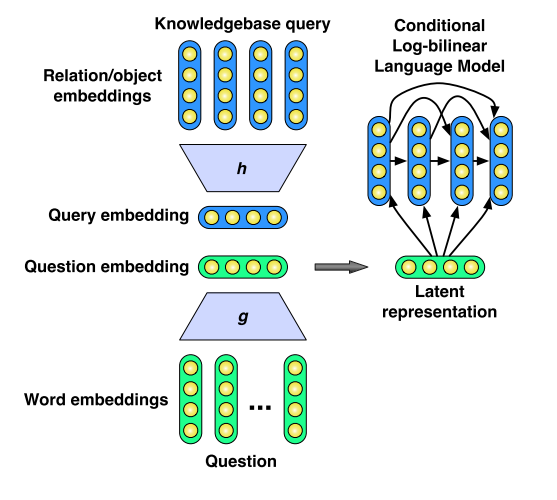
\includegraphics[width=.6\linewidth]{G2014-combined.png}\\
  \caption{Diagrammatic representation of the combined model.}\label{fig:G2014-combined}
\end{figure}

Figure \ref{fig:G2014-combined} shows the combined model. For the natural language side of the model, the composition function $g$ can be a simple additive model. Function $h$, which maps the knowledge base queries into the shared space could use a convolution neural network. Using function $g$ and the original training data, the training data for the second stage is created by obtaining the latent representation for the questions of the original dataset. Once trained, the models can be fully joined to produce a generative neural network.

Finally, the paper suggests that the proposed model can be trained in a two-stage process, and discusses the experimental requirements. However, there is no implementation when the paper is published. So it is left as future work whether the proposed training method can yield fruitful results in practice.
